\documentclass[11pt]{article}
\usepackage[T1]{fontenc}
\usepackage[utf8]{inputenc}
\usepackage{lmodern,microtype,amsmath,booktabs,graphicx,longtable,pdflscape}
\usepackage[margin=1in]{geometry}
\usepackage{xcolor}
\usepackage[colorlinks=true,linkcolor=blue,citecolor=blue,urlcolor=blue]{hyperref}
\usepackage{url}
\usepackage{natbib}
\setlength{\emergencystretch}{2em}
\setlength{\parskip}{0.35em}
\input{generated/macros.tex}
\input{generated/paper_macros.tex}
\makeatletter\let\inputtab\@@input\makeatother
\title{Rank correlation and wavelength error in a fixed Rhomax model panel}
\author{Rewire Bio}
\date{Historical evidence report, 6 October 2026}
\begin{document}
\maketitle
\begin{abstract}
We document a fixed six-configuration panel for peak absorption wavelength on the
FLIP2 Rhomax \texttt{by\_wild\_type} split. The preserved test set contains 184 rows,
with 584 rows used for fitting and 116 held out for validation. Composition features
with a fixed ridge head reach Spearman correlation about 0.418, but their mean
absolute error is \CompMAE\,nm versus \MeanMAE\,nm for a training-mean predictor:
an improvement of only \GainMAE\,nm. The reconstructed-group bootstrap resolves
the direction of that difference while its magnitude remains below the historical
2\,nm reporting threshold. Two frozen ESM-2 configurations have larger point errors;
this is a comparison of fixed configurations, not a tuned comparison of model
families. Candidate selection also depends on the objective: proximity to a desired
wavelength band and maximising wavelength produce different shortlists. All numerical
results in this report are imported from the preserved October 2026 study artifacts.
The manuscript build checks their hashes and formats them; it does not constitute
a new experiment or independent scientific reproduction.
\end{abstract}

\section{Question and scope}
The practical question is whether a model that ranks held-out sequences well also
provides useful wavelength estimates or useful shortlists. These are separate outcomes.
A rank statistic ignores absolute scale, while selecting near a target wavelength
requires predictions whose values have operational meaning.

Rhomax is distributed through FLIP2, which provides explicit splits intended to assess
protein prediction under distribution changes \citep{flip2}. The dataset README
attributes the underlying measurements to \citet{inoue2021}. We use the released
assignment rather than constructing a new split. The endpoint is peak absorption
wavelength in nanometres. No result establishes expression, photostability, ion
transport, activation efficiency or cellular function. There is no new benchwork.

This report preserves the original fixed panel and exploratory analyses. It does not
reinterpret upstream FLIP2 scores as comparable measurements: the archived source
ledger records differences in target-scaling protocol. It also does not infer the
performance of fine-tuned or larger models from the two frozen configurations tested.

\section{Data and fixed methods}
\subsection{Data identity and separation}
The pinned release is labelled \texttt{zenodo-18433203-v3}. Its decompressed CSV has
SHA256 \texttt{8e78f6a1\ldots a65f656f}; the complete digest and retrieval URLs are in
the companion README and source ledger. Gzip framing differs between the mirror and
Zenodo, so decompressed bytes define dataset identity. The CSV provides sequence,
target, set and validation columns. It does not provide per-row wild-type identities,
assay conditions or repeat-measurement identifiers. The upstream split name is therefore
not sufficient to recover labelled biological groups from the CSV alone.

The archived audit reports no exact sequence overlap between the three splits. It also
records duplicate sequences within training, including one pair differing by 19\,nm in
recorded target. This observation is not an estimate of general assay noise, and the
archive does not establish whether the duplicates reflect repeat assays or repackaging.
A supervised separation check also does not establish absence of overlap with the
UniRef pretraining data used for the encoder \citep{esm}. Pretraining exposure remains
undetermined.

\subsection{Predictor configurations}
The constant predictor is the mean of training targets. Composition-22 uses
$\log(1+L)$, 20 residue fractions and an unknown-residue fraction, which is zero on
the pinned alphabet. Composition-40 retains the archived two-component construction:
20 residue fractions followed by 20 zero columns because Rhomax sequences contain no
component delimiter. These are distinct historical configurations; the redundant
columns are retained for fidelity.

The encoder configurations use ESM-2 8M (layer 6, 320 dimensions) and 35M (layer 12,
480 dimensions) \citep{lin2023,esm}. Each sequence is represented by the frozen final-layer
mean over residue positions, excluding start, end and padding tokens. Checkpoint bytes
are pinned before loading. No encoder weights are trained in this panel.

All four feature representations feed a ridge head with $\alpha=10$, an intercept,
solver \texttt{auto}, tolerance $10^{-5}$ and maximum iteration count $10^6$.
Features are not scaled. Targets are standardised using training rows only and mapped
back to nanometres after prediction. Validation and test labels do not participate in
head fitting or historical hyperparameter selection. Equal $\alpha$ does not impose
equal effective regularisation across differently scaled representations.

The additional nearest-sequence control uses normalised Hamming distance among
training sequences of equal length. Ties resolve to the lowest training CSV row.
When there is no equal-length candidate, it predicts the training mean. This control
uses no alignment and treats an insertion or deletion as a length mismatch; its
limitations are intentional and explicit.

\subsection{Metrics and exploratory uncertainty}
We report mean absolute error (MAE), root mean squared error (RMSE), Spearman correlation
and full-ranking NDCG. The NDCG relevance transform subtracts the minimum scored target,
uses linear gains and averages predicted-score ties. Spearman is undefined for a
constant predictor. Its NDCG is defined and can be large without sequence-specific skill.

The historical exploratory protocol reconstructs groups by single linkage among
same-length test sequences at at most 10\% Hamming distance. It yields \Groups\ groups,
including \Singletons\ singletons; the largest has \LargestGroup\ rows. These are declared
sequence clusters, not recovered wild-type labels. Paired bootstrap draws sample whole
groups with replacement and score both predictors on the same sampled rows. The
archived procedure uses \Draws\ draws and seed \BootSeed. The point estimate is the
full-test difference in MAE. A difference is called supported only when the percentile
interval excludes zero and the absolute point difference reaches 2\,nm. This is an
exploratory reporting rule, not a multiplicity-adjusted confirmatory test, an equivalence
test, or a universally justified biological tolerance.

\section{Results}
\subsection{Rank advantage is a small error reduction}
Table~\ref{tab:main} records all configurations. Composition-22 reduces MAE by
\GainMAE\,nm relative to the constant. Its paired 95\% bootstrap interval for
candidate-minus-constant MAE is approximately $[-0.45,-0.05]$\,nm, below zero but below
the 2\,nm reporting threshold in magnitude. Composition-40 behaves almost identically.
A positive rank correlation alone therefore overstates the benefit for numerical
wavelength estimation on this split.

\begin{table}[htbp]\centering\small
\caption{Historical held-out results on 184 test rows. Undefined correlation is not zero.}\label{tab:main}
\begin{tabular}{lrrrr}\toprule
Configuration & MAE (nm) & RMSE (nm) & Spearman & NDCG\\\midrule
\inputtab{generated/tab_main_compact.tex}
\bottomrule\end{tabular}
\end{table}

The two frozen ESM-2 configurations have larger MAE point estimates than the constant.
Only the 35M configuration meets both parts of the historical difference rule; the 8M
interval crosses zero. The nearest-sequence control also has an interval spanning zero.
None of those intervals establishes equivalence. The panel does not select a tuned
representation, tune ridge regularisation, or compare a common effective penalty.

The composition prediction spread explains the gap between ranking and numerical
accuracy (Table~\ref{tab:spread}). Composition-22 spans about 2.2\,nm while the measured
test standard deviation is about 32.15\,nm. A narrow prediction distribution may order
some rows while remaining close to a constant. The archived scale diagnostics also
show that representation variances differ substantially under the same ridge penalty.

\begin{figure}[htbp]\centering
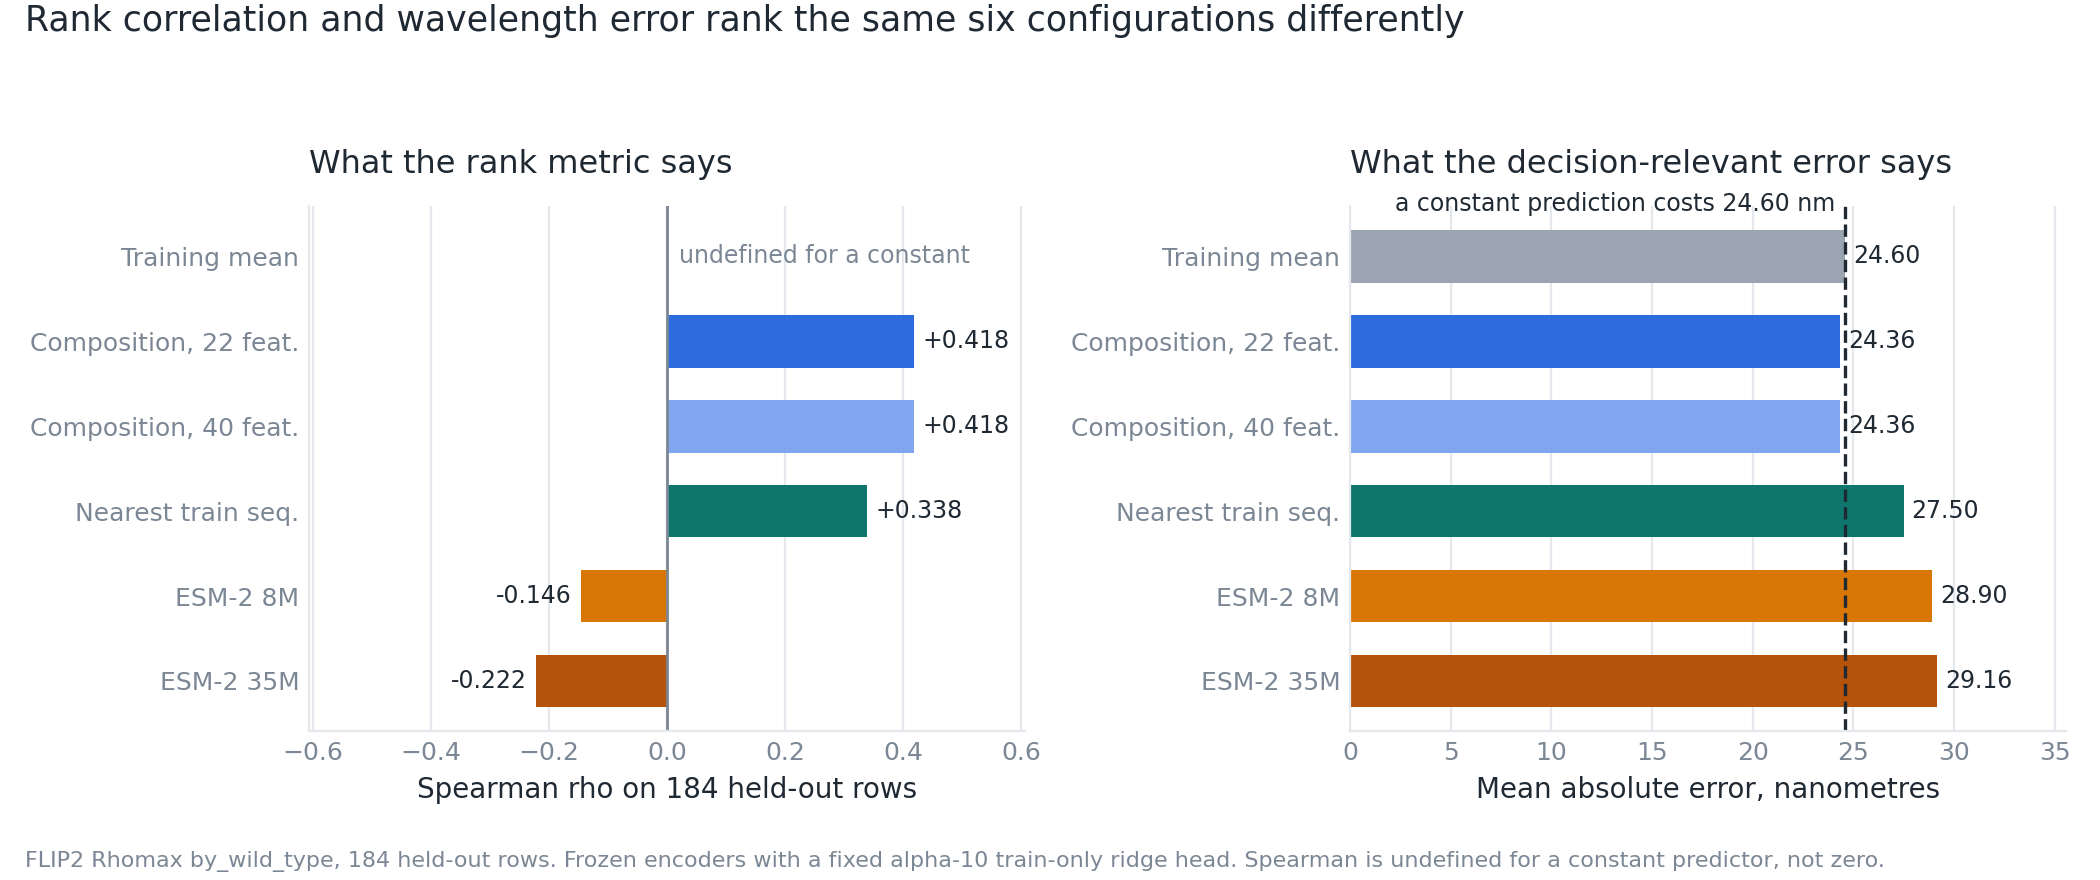
\includegraphics[width=0.95\linewidth]{../article/assets/01-rank-versus-error.png}
\caption{Original preserved rank-versus-error figure. Values describe the fixed historical panel.}
\end{figure}

\subsection{Distance strata are descriptive}
The fixed distance bins are near ($d\leq0.05$), mid ($0.05<d\leq0.25$), far
($0.25<d<1$), and no equal-length training sequence. There are \Fallbacks\ test rows
in the final category. The near bin has only five rows; no row lies in the mid bin. The nearest-sequence control has
the smallest near-bin MAE, while errors increase in more distant strata. Those
within-bin comparisons have no paired interval and are descriptive, even when their
row count meets the minimum of ten. The length gate can classify a close indel variant
as lacking a neighbour, so the strata are not a general homology measure.

\begin{figure}[htbp]\centering
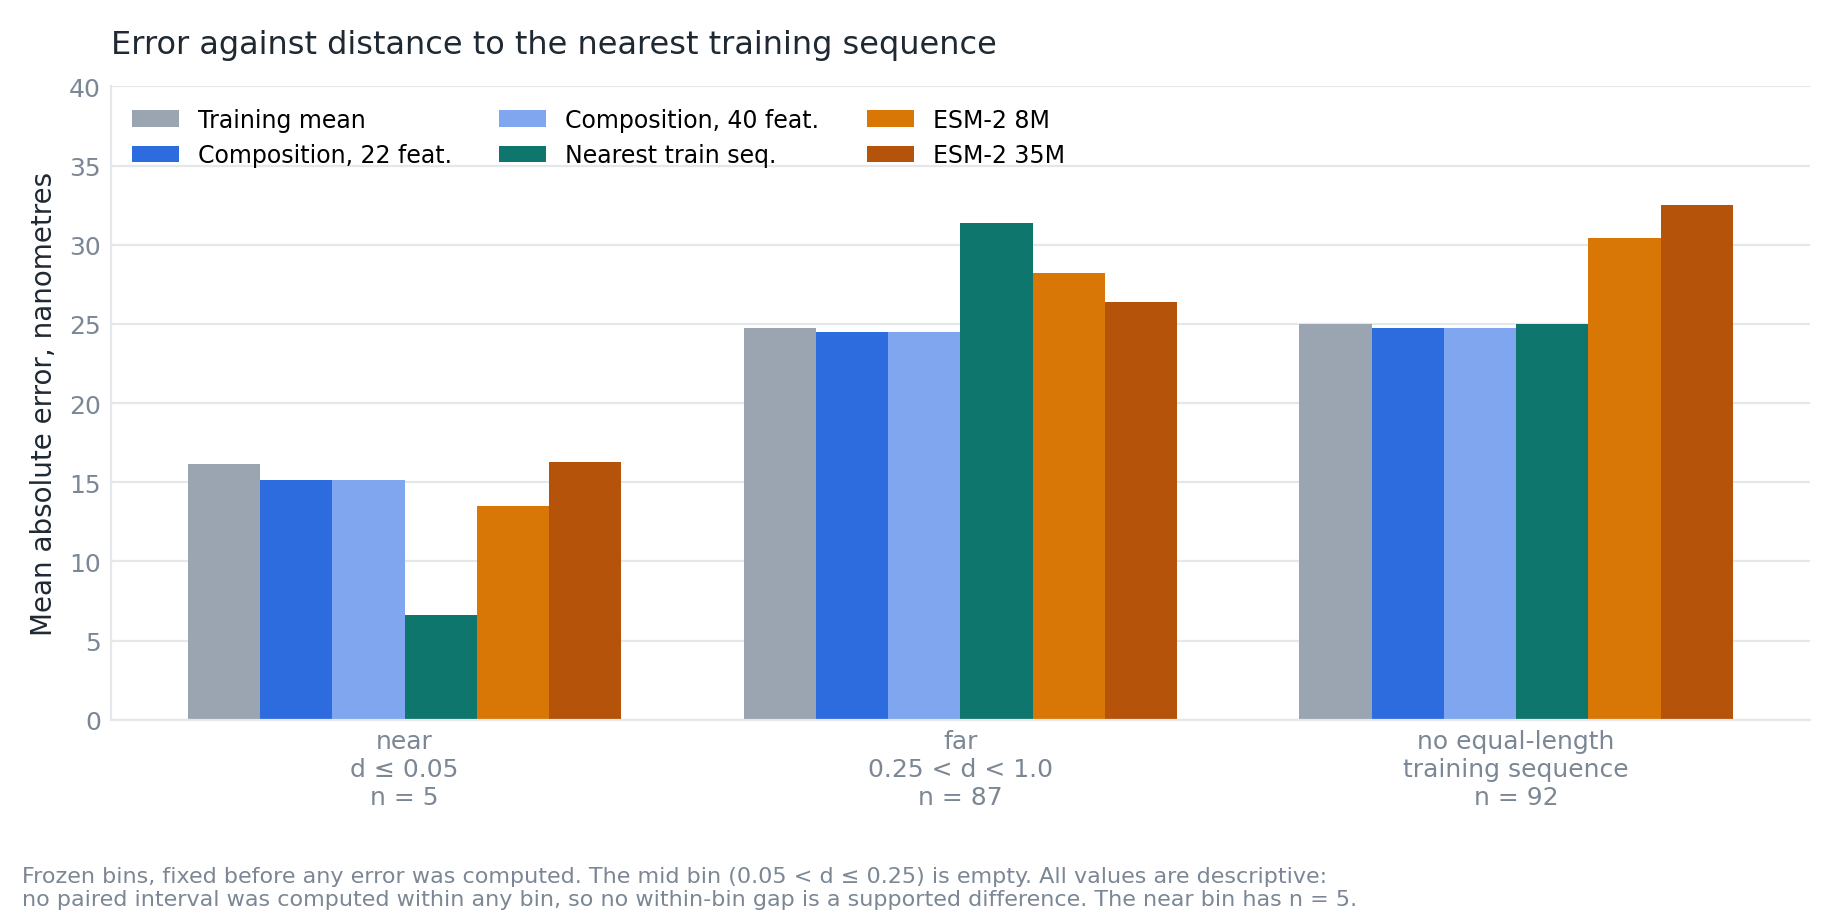
\includegraphics[width=0.95\linewidth]{../article/assets/03-distance-bins.png}
\caption{Original descriptive distance-stratum results. Absence of within-bin uncertainty limits comparative claims.}
\end{figure}

\subsection{Two shortlist objectives}
Decision A selects ten rows with predictions closest to 550\,nm and measures the
fraction whose observed wavelengths lie in $[540,560]$\,nm. Decision B selects the
ten largest predictions and reports their mean observed wavelength. Ties use stable
CSV order. A constant predictor has no defined shortlist under this policy.

Composition-22 puts 9 of 10 selected rows in the desired band, compared with an analytic
uniform-random expectation of about 0.310. Its red-shift shortlist has mean measured
wavelength 553.50\,nm. These are different estimands; neither alone establishes accurate
individual predictions. The post-hoc shortlist bootstrap resamples reconstructed groups
and holds shortlist fraction fixed, so the realised depth varies from
\ShortlistDepthMin\ to \ShortlistDepthMax\ for Composition-22. The resulting intervals
are exploratory spreads, not repeated independent tests of a ten-sequence intervention.

A high-wavelength hit among ten candidates is also not sufficient evidence of skill.
The archived finite-population calculation gives approximately 0.3283 probability
that a uniform random ten-row shortlist includes at least one observation at or above
580\,nm. This comparison conditions on the existing test population and does not predict
prospective laboratory success.

\begin{figure}[htbp]\centering
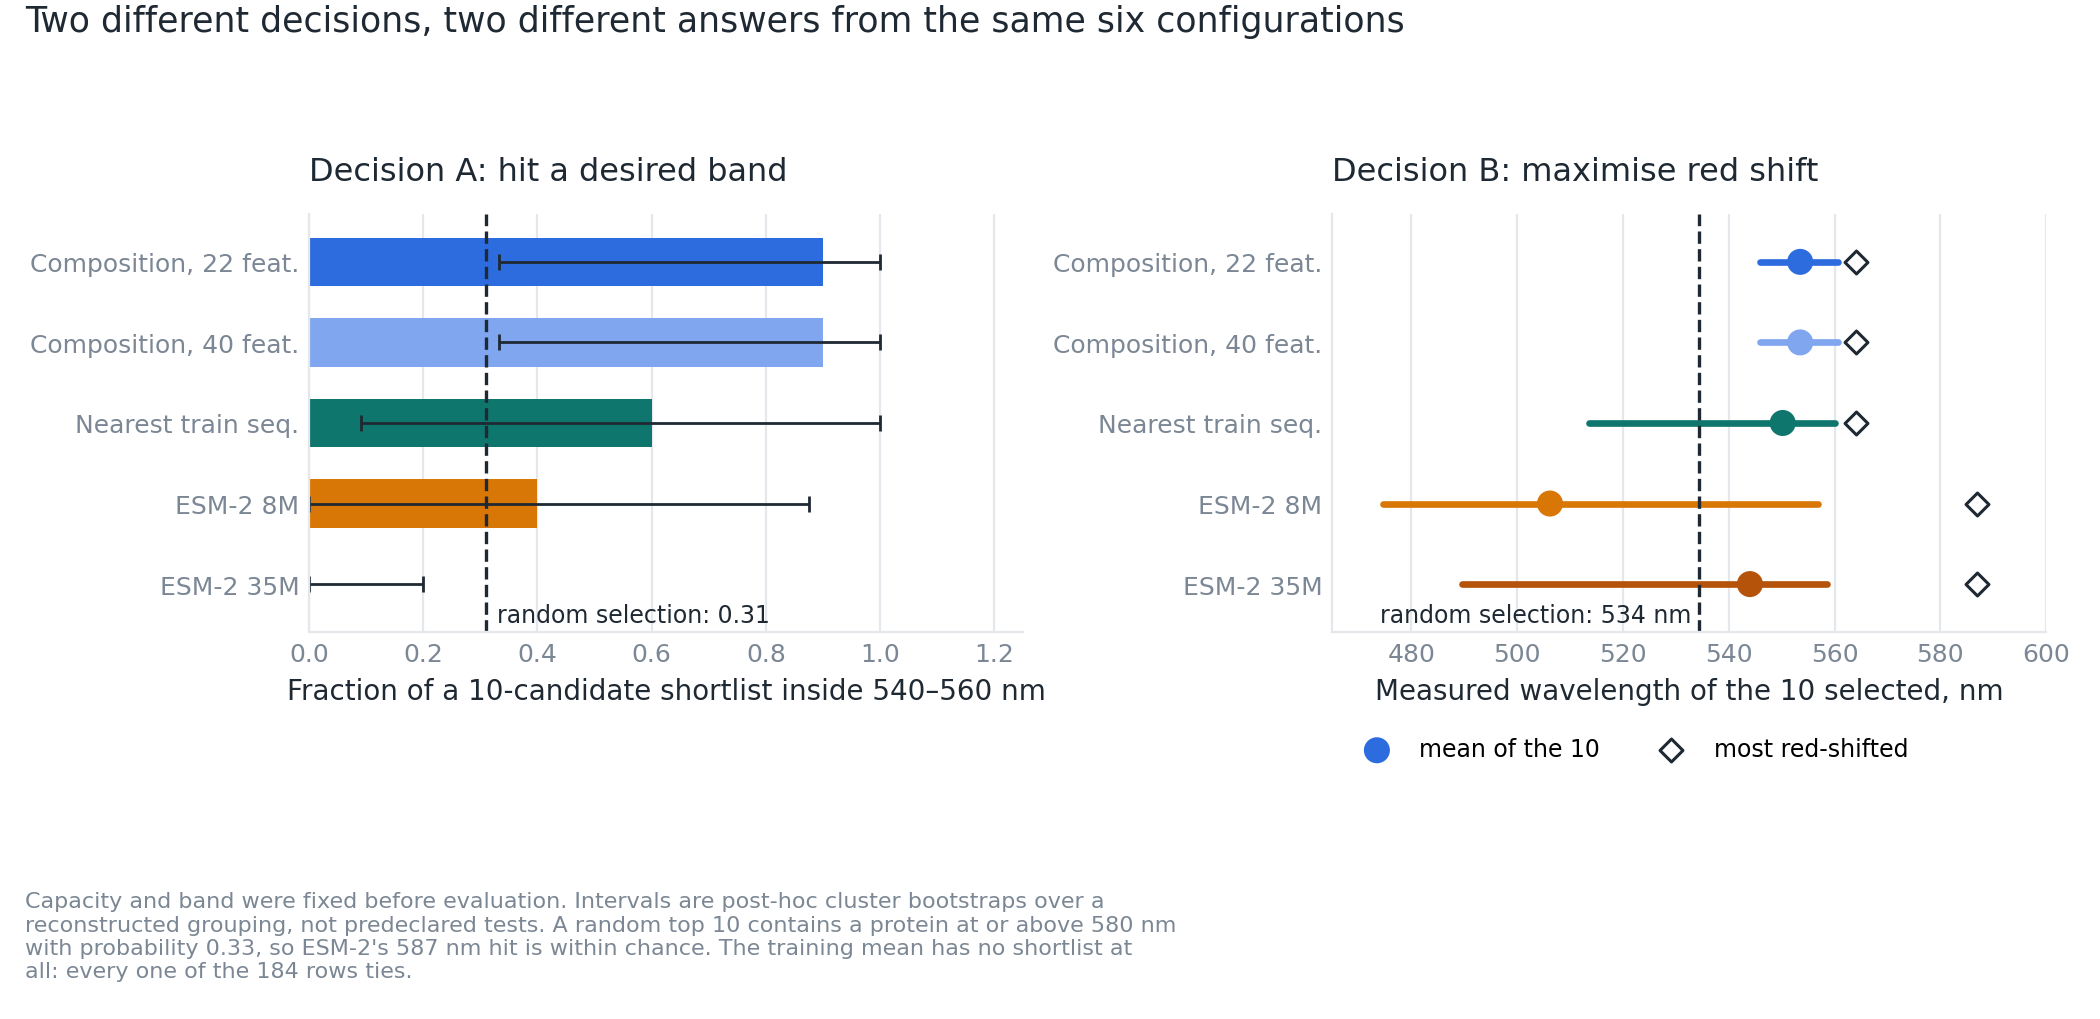
\includegraphics[width=0.95\linewidth]{../article/assets/04-two-decisions.png}
\caption{Original shortlist figure. Desired-band precision and mean selected wavelength answer different questions.}
\end{figure}

\subsection{Post-hoc interval feasibility}
The preserved probe sets a symmetric half-width to the empirical 90th percentile of
absolute validation residuals, using the higher order-statistic interpolation rule.
It then reports test coverage. The procedure is descriptive; it is not asserted to be
an exact finite-sample conformal interval. Observed coverage is below the nominal 90\%
for every configuration (Table~\ref{tab:probe}). Row-level Wilson intervals are retained
for fidelity, but their independent-row assumption does not account for reconstructed
group dependence. They must not be interpreted as background-level coverage guarantees.
The validation set is a single held-out collection, so coverage under new background
shifts remains unestablished.

\section{Limitations and interpretation}
The main conclusion is conditional: on this split and these fixed configurations, the
composition ranking advantage buys little absolute-error improvement over a constant.
The evidence does not imply that protein language models are generally inferior, that
ridge is optimally regularised here, or that the preferred shortlist transfers to a new
assay. The bounded panel lacks alignment-based controls, tuned or fine-tuned models,
repeated labelled background splits and a prospective experimental validation.

Missing wild-type and assay metadata restrict causal interpretation of error differences.
Single-linkage reconstructed groups can join chains of near neighbours and are an
imperfect dependence model. No adjusted family-wise significance claim is made across
the multiple model comparisons. The observed results cannot separate measurement
variation, representation limitations and distribution shift into independent effects.

A future study could predeclare model tuning, an alignment policy, independent
background evaluation and a decision-specific utility measure. Those are proposals;
no such experiment is reported here.

\section{Provenance, maintenance and availability}
The repository preserves the original detailed article, published text, figures,
code archive and result archive. Two original prediction NPZ files omitted from the
published tarball were subsequently recovered unchanged; their recovery manifest
records hashes and byte identity with the retained run directory. The publication
archives themselves remain unchanged.

The archived receipt records a historical reimplementation matching the earlier five
configuration rank metrics. This manuscript reports that receipt as historical evidence;
it does not convert it into a new independent reproduction of the current repository.
The current paper build verifies archive and member digests, checks printed article
values, generates tables and compiles this document. The generated claim ledger maps
findings to archived JSON fields. No training or new scientific analysis is required
for the build. The current root research harness remains unapproved and disabled.

The October 2026 maintenance audit repaired installation portability, test coverage,
invalid numeric arguments, prediction metadata checks and embedding cache provenance.
Those guards do not change the historical settings or measurements. Existing caches
without provenance require an explicit refresh before future use. Original downloaded
code remains an archival snapshot; current execution instructions live in the maintained
companion README.

All source measurements retain upstream licensing and attribution. Checkpoints are
retrieved from upstream sources and are not redistributed. Repository materials are at
\url{https://github.com/rewire-bio/rhodopsin-model-selection}.

\clearpage
\bibliographystyle{plainnat}
\bibliography{references}

\clearpage\appendix
\begin{landscape}
\section{Complete numerical supplement}
The following tables are generated directly from the preserved result archive. No
original result artifact is dropped: the mapping in
\texttt{evidence/paper-migration-map.json} identifies original tables, figures and
supplemental files. The detailed original article remains available for its full
historical narrative and bibliography.

\begin{table}[htbp]\centering\scriptsize
\caption{Full panel and historical paired difference interpretation. MAE differences are candidate minus training mean.}
\begin{tabular}{p{4.2cm}rrrrrp{2.8cm}p{4.1cm}}\toprule
Configuration & Spearman & NDCG & MAE & RMSE & $\Delta$MAE & 95\% interval & Interpretation\\\midrule
\inputtab{generated/tab_panel.tex}
\bottomrule\end{tabular}
\end{table}
\end{landscape}

\begin{table}[htbp]\centering\small
\caption{Prediction spread; the measured test standard deviation is 32.15\,nm.}\label{tab:spread}
\begin{tabular}{lrrrr}\toprule
Configuration & SD (nm) & Span (nm) & SD/measured & Pearson\\\midrule
\inputtab{generated/tab_spread.tex}
\bottomrule\end{tabular}
\end{table}

\begin{table}[htbp]\centering\small
\caption{Representation scales under the same $\alpha=10$. This is not equal effective regularisation.}
\begin{tabular}{lrrrr}\toprule
Representation & Dimension & Zero columns & Total variance & Variance/$\alpha$\\\midrule
\inputtab{generated/tab_regularisation.tex}
\bottomrule\end{tabular}
\end{table}

\begin{table}[htbp]\centering\small
\caption{Desired-band shortlist. Spread intervals are post hoc; random selection is an analytic expectation.}
\begin{tabular}{lrrrr}\toprule
Configuration & In band & Precision & Deviation (nm) & 95\% spread\\\midrule
\inputtab{generated/tab_decisionA.tex}
\bottomrule\end{tabular}
\end{table}

\begin{table}[htbp]\centering\small
\caption{Red-shift shortlist. The oracle is a retrospective upper bound, not a deployable predictor.}
\begin{tabular}{lrrr}\toprule
Configuration & Mean (nm) & Maximum (nm) & 95\% spread (nm)\\\midrule
\inputtab{generated/tab_decisionB.tex}
\bottomrule\end{tabular}
\end{table}

\begin{table}[htbp]\centering\small
\caption{Archived validation-residual interval feasibility. Wilson intervals treat rows as independent and are descriptive only.}\label{tab:probe}
\begin{tabular}{lrrrr}\toprule
Configuration & Half-width (nm) & Coverage & Wilson 95\% & Nominal\\\midrule
\inputtab{generated/tab_probe.tex}
\bottomrule\end{tabular}
\end{table}

\begin{landscape}
\begin{table}[htbp]\centering\small
\caption{Distance bins and descriptive MAE (nm). Composition-40 agrees with Composition-22 at the shown precision.}
\begin{tabular}{p{4.5cm}rrr rrrrr}\toprule
Bin & $n$ & $n\ge10$ & Target range & Nearest & ESM-8M & Comp.-22 & Constant & ESM-35M\\\midrule
\inputtab{generated/tab_bins.tex}
\bottomrule\end{tabular}
\end{table}
\end{landscape}

\begin{landscape}
\begin{table}[htbp]\centering\scriptsize
\caption{Example test rows from the original article. Digests are local sequence identifiers, not accessions. All wavelengths are in nm.}
\begin{tabular}{lrrrllrrr}\toprule
Sequence digest & CSV row & Length & Measured & Distance & Neighbour digest & Nearest & Comp.-22 & ESM-35M\\\midrule
\inputtab{generated/tab_rows.tex}
\bottomrule\end{tabular}
\end{table}
\end{landscape}

\begin{landscape}
\begin{table}[htbp]\centering\small
\caption{Paired reconstructed-group bootstrap details. The reporting threshold is 2\,nm in absolute point difference.}
\begin{tabular}{lrrr rrrr}\toprule
Configuration & $\Delta$MAE & 95\% interval & Bias & Fraction better & Excludes 0 & Meets 2\,nm & Supported\\\midrule
\inputtab{generated/tab_bootstrap.tex}
\bottomrule\end{tabular}
\end{table}
\end{landscape}

\clearpage
\begin{center}\small
\begin{longtable}{lrrrrrr}
\caption{Per-reconstructed-group MAE (nm), descriptive only.}\\
\toprule Group & $n$ & Constant & Comp.-22 & Nearest & ESM-8M & ESM-35M\\\midrule\endfirsthead
\toprule Group & $n$ & Constant & Comp.-22 & Nearest & ESM-8M & ESM-35M\\\midrule\endhead
\inputtab{generated/tab_groups.tex}
\bottomrule
\end{longtable}
\end{center}

\begin{table}[htbp]\centering\small
\caption{Historical reproduction receipt: archived rank metrics and differences reported by the original companion run. Not a new reproduction.}
\begin{tabular}{lrrrrl}\toprule
Configuration & Spearman & Difference & NDCG & Difference & Status\\\midrule
\inputtab{generated/tab_repro.tex}
\bottomrule\end{tabular}
\end{table}

\begin{table}[htbp]\centering\small
\caption{Historical single-run feature/embedding and fit/prediction times (seconds). The receipt reports \WallSeconds\,s total and \PeakRSS\,GiB peak RSS.}
\begin{tabular}{lrr}\toprule
Configuration & Features/embedding & Fit/predict\\\midrule
\inputtab{generated/tab_timings.tex}
\bottomrule\end{tabular}
\end{table}

\begin{table}[htbp]\centering\small
\caption{Finite-population random shortlist references, capacity ten of 184.}
\begin{tabular}{lrr}\toprule
Threshold & Population hits & Probability of at least one\\\midrule
\inputtab{generated/tab_chance.tex}
\bottomrule\end{tabular}
\end{table}

\begin{landscape}
\begin{table}[htbp]\centering\small
\caption{Measured wavelengths in the original red-shift shortlists, in predicted rank order.}
\begin{tabular}{lrrrrrrrrrr}\toprule
Configuration & 1 & 2 & 3 & 4 & 5 & 6 & 7 & 8 & 9 & 10\\\midrule
\inputtab{generated/tab_shortlistB.tex}
\bottomrule\end{tabular}
\end{table}
\end{landscape}

\clearpage
\section{Additional preserved diagnostics}
The NDCG finite-population reference gives reverse-order score \NdcgWorst, random
permutation mean \NdcgRandMean\ and percentile range $[\NdcgRandLo,\NdcgRandHi]$ across
\NdcgDraws\ draws (seed \NdcgSeed). These are preserved diagnostics, not new permutation
tests. The exact constant-score NDCG is determined by tie averaging and the observed
label distribution.

The archived environment records Python \EnvPython, NumPy \EnvNumpy, SciPy \EnvScipy,
scikit-learn \EnvSklearn\ and torch \EnvTorch. A historical CPU/MPS embedding comparison
on \DeviceSeqs\ sequences recorded maximum absolute difference \DeviceMaxDiff;
that small device check is not a full cross-platform reproduction.

\begin{figure}[htbp]\centering
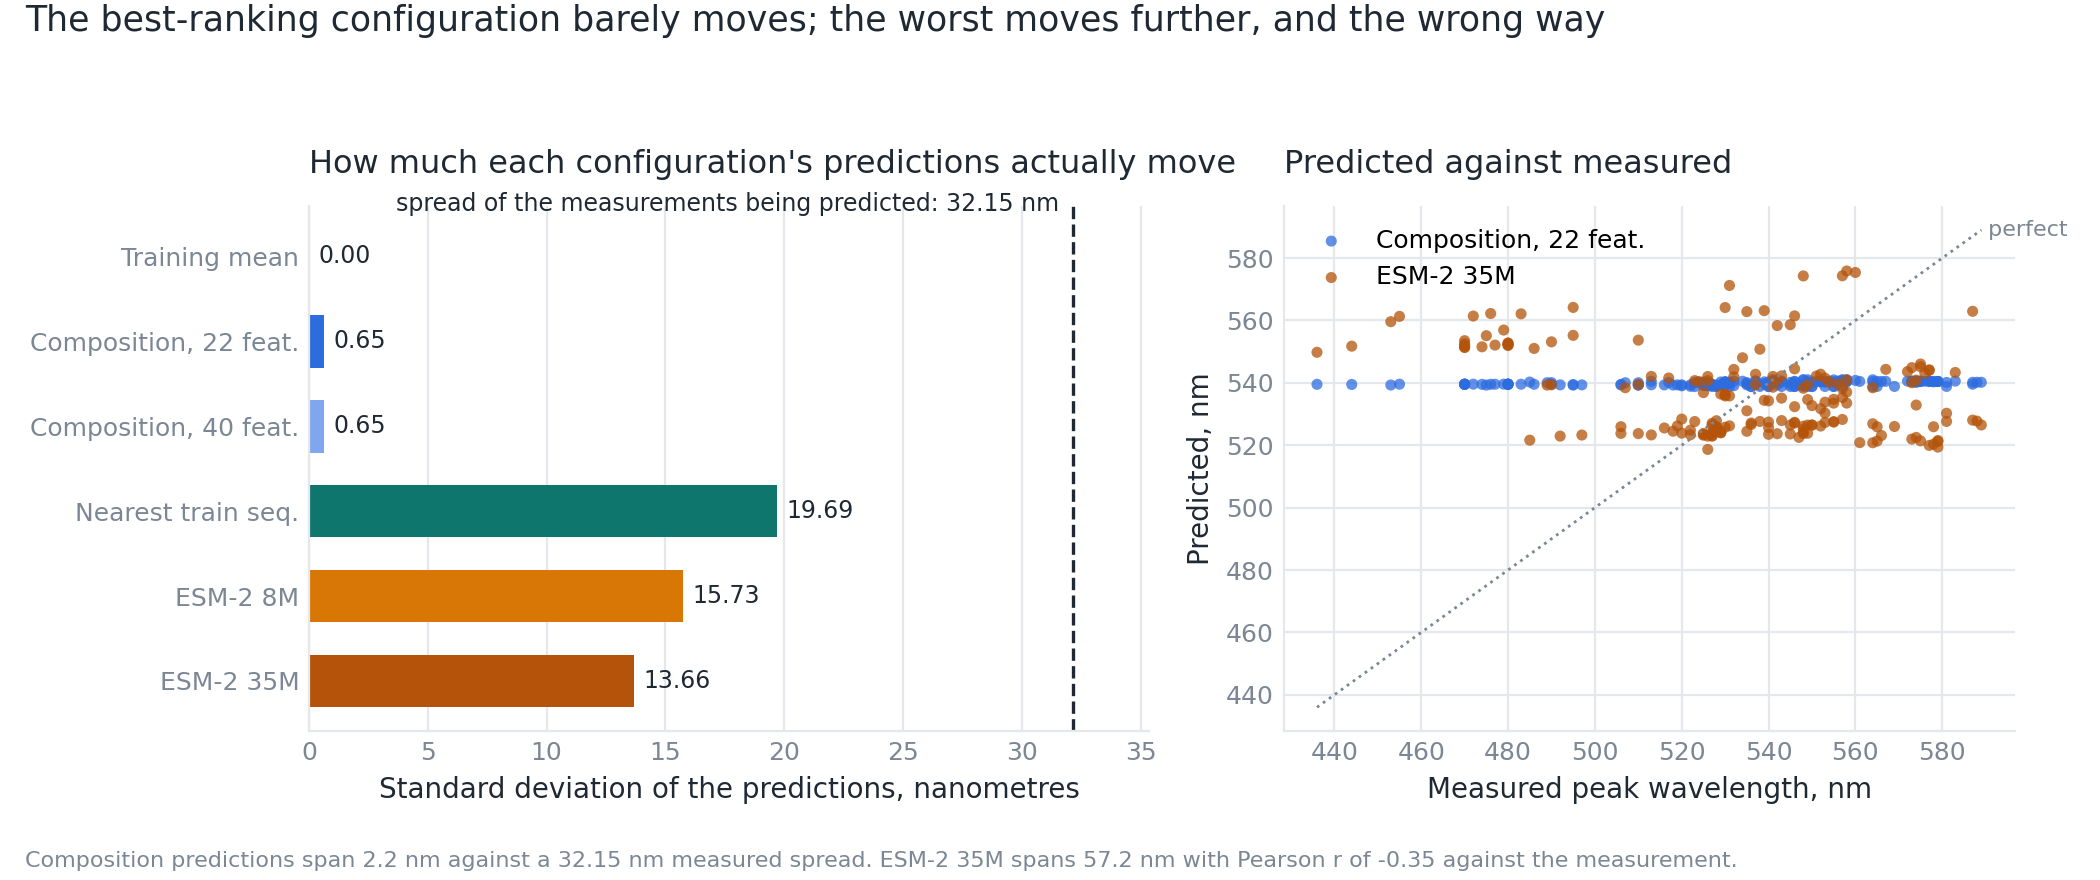
\includegraphics[width=0.95\linewidth]{../article/assets/02-prediction-spread.png}
\caption{Original preserved prediction-spread figure. The source SVG decision diagram and its D2 source remain in the archive mapping.}
\end{figure}
\end{document}
